\section{Gaifman locality}\label{sec:gaifman}
In this section, we extract from Gaifman's Locality Theorem~\cite{gaifman1982local} a technical lemma
(\cref{pro:crossing} below), which will be used later on two different occasions (in the proofs of~\cref{thm:uqw-stable} and
of~\cref{thm:vc-density}).



If $X,Y,S\subset V(G)$ are sets of vertices of a graph $G$ 
and $r\in \N$, then we say that $X$ and $Y$ are  \emph{$r$-separated}
by $S$  (in $G$) if every path between a vertex in $X$ and a vertex in 
$Y$ of length at most~$r$ contains a vertex from $S$. If $G$ is a graph, $B\subset V(G)$ is a set of vertices,
and $v,w\in V(G)^d$ are two tuples of vertices, then we say that 
$v$ and $w$ have \emph{the same quantifier rank $q$ type} over $B$
if $v$ and $w$ satisfy exactly the same formulas of quantifier rank $q$ with parameters from $B$.



The aim of this section is to prove the following technical lemma, which
may be considered folklore (cf. Fig~\ref{fig:gaifman} for a graphical illustration). 


\begin{lemma}\label{pro:crossing}	
	% Let $\phi$ be a formula with
	%  quantifier rank $q$ and
	%    free variables $X$
	%  partitioned as $X=Y\cup Z$.
For
every graph $G$, set of vertices $S\subset V(G)$, integers $q,d\in\N$, 
there is a  function mapping tuples  $v\in V(G)^d$
	to \emph{$(q,S)$-local types},
so that the following conditions 
hold.
	 \begin{enumerate}[(1)]
	 	\item\label{c:number} The  set of  $(q,S)$-local types  of all tuples $v\in V(G)^d$  has at most
    $T(q,d,|S|)$ elements, for some computable function $T\from \N\times \N\times\N\to \N$ which is weakly increasing in all of its arguments.

	
		
    % \item The $\phi$-type of $v\in V(G)^X$ only depends on the pair $(H,v)$, where $H$ is the subgraph induced by the vertices in $G$
    %     which are within distance at most  $r(q)$  from some vertex in the range of $v$, for some computable function $r(\cdot)$.

		
	 	\item\label{c:confusing}
		 % 	    Let $\phi$ be a formula with
		 % 	   	 quantifier rank $q$,
		 % parameters from $K\subset V(G)$, and free variables $Y$.
		 	  There is a number 
		 $r\in\N$ computable from $q$ with the following property. 
		 If $A,B\subset V(G)$ are 
 $r$-separated by $S$,
then any two tuples $u,v\in A^d$
		 of the same $(q,S)$-local type
have
		 the same  quantifier rank $q$ type
		 over $B$.
		 	%
	%
	%   if $u,v\in V(G)^Y,w\in V(G)^Z$ satisfy:
	%   \begin{itemize}
	% \item  $u$ and $w$ are $r$-independent in $G-S$,
	% \item  $v$ and $w$ are $r$-independent in $G-S$, and
	%   	\item $u$ and $v$ have the same $(q,S,Y)$-types,
	%   \end{itemize}
	%   then
% \[G,u\oplus w\models \phi\iff G,v\oplus w\models \phi.\]
	 \end{enumerate}
\end{lemma}

\begin{figure}[h!]
	\centering
		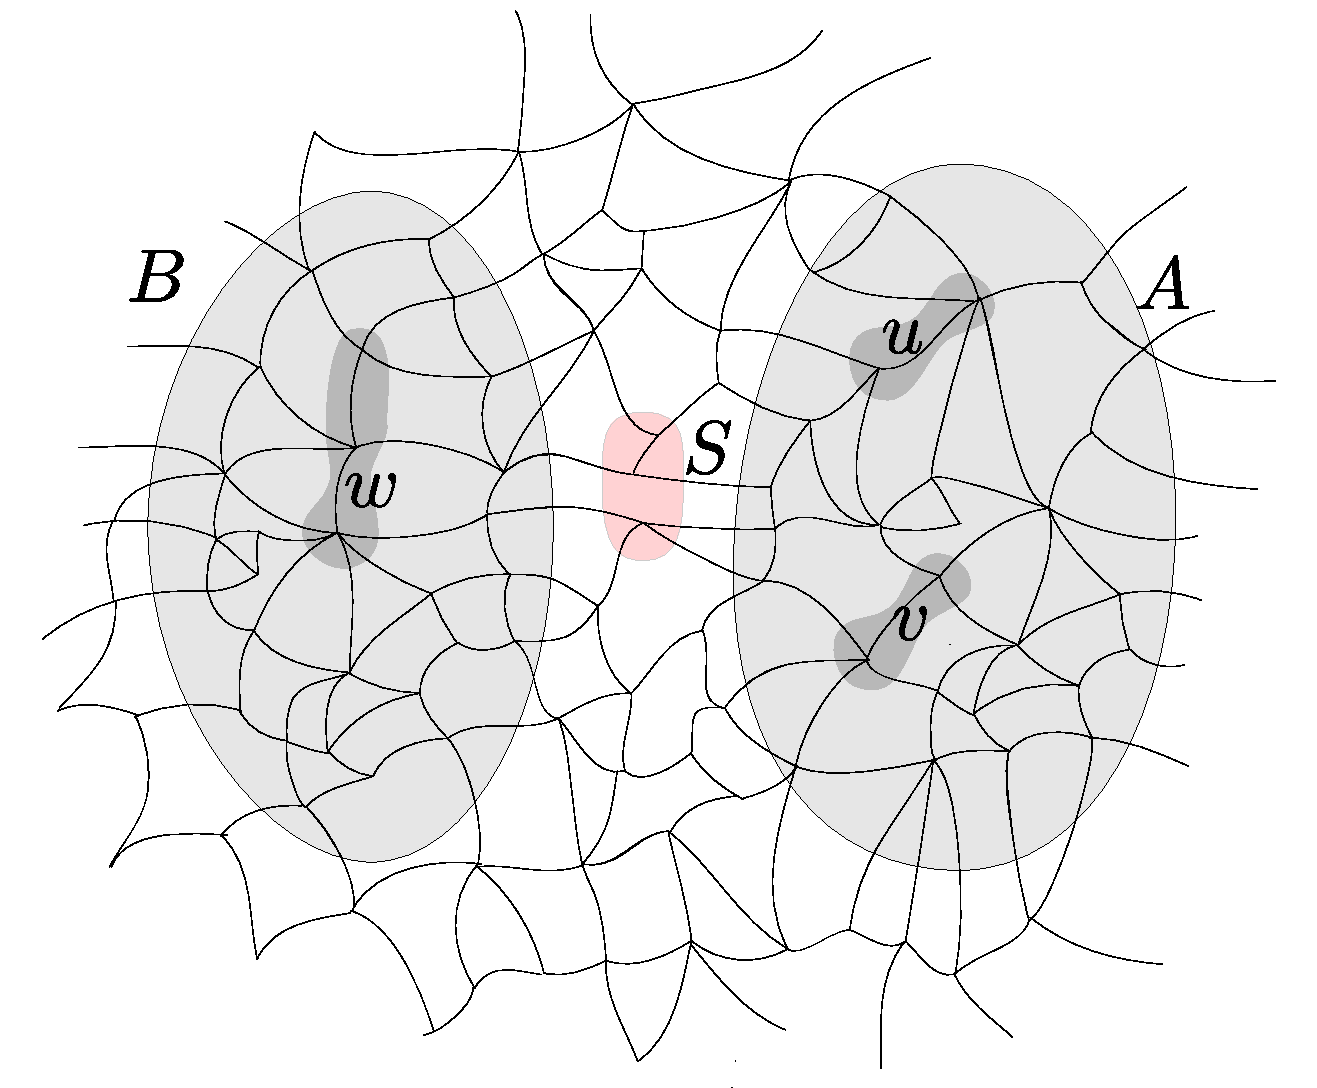
\includegraphics[scale=0.3,page=1]{pics}
	\caption{The sets $A$ and $B$ are $r$-separated by $S$
	(here $r=3$), and the tuples $u,v$ of elements of $A$ are assumed to have  
	the same \emph{$(q,S)$-local type}, where $q\sim \log r$. This implies that 
	for every first-order formula $\phi(\bar x,\bar y)$ of quantifier rank
	$q$
	(where $|\bar x|=|u|=|v|$)
	and every tuple $w$ of $|\bar y|$ elements of $B$,	
	  $\phi(u,w)$ holds in $G$ iff 
	 $\phi(v,w)$ holds in $G$.
	}
	\label{fig:gaifman}
\end{figure}

The rest of Section~\ref{sec:gaifman} is devoted to the proof of~\cref{pro:crossing}.
We start by introducing some notation which will be used in this proof only.

We consider only finite sets of variables, and any mathematical object can be considered a variable 
(formally, whenever we want to treat an object $a$ as a variable, we introduce a variable~$x_a$, where~$x$ is a fixed special symbol).
If $\phi$ is a formula then it has a specified set of free variables.
By abuse of language, if $X$ is a set of variables and $\phi$
is a formula, when we say that $\phi$ \emph{has free variables}~$X$
we allow the set of free variables of $\phi$ to be a subset of $X$.

If $X$ is a finite set and $V$ is a set, then $V^X$ denotes the set of functions from $X$ to $V$, and an element $v\in V^X$ will be sometimes called a \emph{tuple} 
or, in the case $X$ is a set of variables, a \emph{valuation} of $X$.
For two tuples
$v\in V^Y$ and $w\in  W^Z$, where $Y$ and $Z$ are disjoint, by
$v\oplus w$ we denote the set-theoretic union of the functions $v,w$,
which is a tuple $v\oplus w\in (V\cup W)^{Y\cup Z}$.
The image of a valuation $v$ is denoted by $\im(v)$.


% If $V=V(G)$ for some graph $G$, then we can treat valuations of~$X$ as tuples of length $|X|$ consisting of vertices of $G$, ordered in the same way according to any fixed enumeration of $X$.
% Then we may say that a set of valuations is mutually $r$-independent in~$G$, or in $G-S$ for some $S\subseteq V(G)$, meaning the notion discussed in the previous section.


Fix a formula $\phi$ with free variables $X$.
Given a valuation $v\in V(G)^X$, we write $G,v\models \phi$ to denote that $\phi$ is satisfied 
in the graph $G$ with valuation $v$, which is defined as usual in logic, by induction on the structure of $\phi$.




It remains to prove~\cref{pro:crossing}. 
First we recall some notions from logic, namely quantifier ranks, Gaifman's Locality Theorem, and some simple manipulations on formulas.

 Fix a finite set of  colors $C$.
By a \emph{colored graph} we mean a graph  in which 
every vertex is assigned zero or more colors from $C$. We view a colored graph as a relational structure as usual, by treating each color as a unary predicate. 

The \emph{quantifier rank} of a formula $\phi$ is the maximal number of nested quantifiers in $\phi$.
For $i=1,2$, let $G_i$
be a colored graph and $v_i:X\to V(G_i)$ be a valuation
from a common set of variables $X$.
We say that $(G_1, v_1)$ and $(G_2,v_2)$
have the same \emph{quantifier rank $q$ type} %\marginpar{also called $q$-equivalent and denoted $(G_1,\bar v_1)\equiv_q (G_2, \bar v_2)$}
if for every formula $\phi$ with  free variables $X$ and of quantifier rank $q$,
 $$G_1,v_1\models \phi\qquad\iff \qquad G_2,v_2\models \phi.$$
If $G$ is a graph colored with colors from $C$ and 
 $v\from X\to V(G)$ is a valuation, 
then the equivalence class of $(G, v)$ under the above equivalence relation is called the \emph{quantifier rank $q$ type} of $(G,v)$, and  the set of \emph{quantifier rank $q$ types with  free variables $X$}
is the set of all equivalence classes, denoted
$\mathrm{Tp}^{q,C}_X$.

 If $G$ is a colored graph, $r\in\N$ is an integer, and $v$ is a valuation of a set of variables in $G$, then  $N^G_r[v]$ denotes the pair $(H,v)$, where $H$ is the colored subgraph of $G$
induced by the set of all vertices which are in distance at most $r$
from some vertex in the image of $v$.
If $r$ is an integer, then the \emph{$(r,q)$-local type} of $(G,v)$ is 
the quantifier rank $q$ type of $N^G_r[v]$. The $q$-\emph{local type} of $(G,v)$ is the $(r,q)$-local type, where $r$   is the value described in the second item of the following proposition,  summarizing several well-known properties of types and local types.


\begin{proposition}\label{pro:gaifman}
	Fix a positive integer $q$, a finite set of colors $C$, and a set of variables $X$. Let~$G$ be any $C$-colored graph. Then the following conditions hold:
 \begin{enumerate}[(1)]
 	\item \emph{(Computability of types)} The set of types $\mathrm{Tp}^{q,C}_X$ is finite and computable from $C$, $X$, and $q$.

	\item \emph{(Locality of first order logic)} There is an integer $r$ computable from $q$ such that for every formula $\phi$ in the signature of $C$-colored graphs  
	of quantifier rank $q$ and with free variables~$X$,	
  if $(G,v_1)$ and $(G,v_2)$ have the same $(r,q)$-local types,
	then
	 $$G,v_1\models \phi\qquad\iff \qquad G,v_2\models \phi.$$
   % We call $r$ the \emph{locality radius} for quantifier rank $q$, and fix this number in what follows.

%    \item \emph{(Monotonicity)} If $Y\subset X$ and $v \from X\to V(G)$
%    is a valuation, then the $(q,r)$-local type of $(G,v)$
% determines   the $(q,r)$-local type $(G,v|_Y)$ of the restriction of $v$ to $Y$.


	 \item \emph{(Independence)} Suppose $X$ is partitioned into $Y\cup Z$, 
	 and that $u_1,u_2\from Y\to V(G)$ and $v_1,v_2\from Z\to V(G)$ are valuations
   such that  $u_1$ and $v_1$, as well as $u_2$ and $v_2$,
   are $2r$-independent in $G$, for some $r$.
   Moreover, suppose that the $(r,q)$-local types of $(G,\im(u_1))$ and $(G,\im(u_2))$ are equal,
   and that the $(r,q)$-local types of $(G,\im(v_1))$ and $(G,\im(v_2))$ are equal.
   Then the $(r,q)$-local types of $(G,u_1\oplus v_1)$ and $(G,u_2\oplus v_2)$ are equal.
 \end{enumerate}
\end{proposition}


\begin{proof}%[of~\cref{pro:gaifman}]

\emph{Computability of types} is standard~(see e.g. Lemma 3.13 in~\cite{libkin}).
% and  yields the first condition in~\cref{pro:gaifman}.
% \begin{lemma}\label{lem:q-types}
%   Fix a set of colors $C$, a rank $q$ and a set of variables $X$.
%   Then the set $\mathrm{Tp}^{q,C}_X$ of quantifier rank $q$ types with free variables $X$ is finite and computable.
% \end{lemma}

\emph{Locality of first order logic} is an
immediate consequence of Gaifman's Locality Theorem
(the Main Theorem~in~\cite{gaifman1982local}),
where it is shown that one can take $r=7^q$.
It is also known (cf. Exercise~4.10 in \cite{libkin}) that it suffices to take $r=2^q$; this bound is tight.


% We say that a formula $\phi(\bar x)$ with $d=|\bar x|$ free variables is \emph{$q$-local} if for every colored graph $G$ and every $\bar a_1,\bar a_2\in V(G^d)$, if  $N^G_r(\bar a_1)$ and  $N^G_r(\bar a_2)$
% are isomorphic, then $G,\bar a_1\models \phi(\bar x)$ if and only if $G,\bar a_2\models \phi(\bar x)$.
%
% \begin{lemma}\label{lem:gaifman}
%   Let $\phi$ be a  formula
%   of quantifier rank $q$
%   in the signature of colored graphs, with free variables $X$.
%   Suppose $v_1,v_2$ are valuations of $X$ in $G$ such that $N^G_r[v_1]$ and $N^G_r[v_2]$ have the same quantifier rank $q$ type, where $r=7^q$. Then
%  $$G,v_1\models \phi\qquad\iff \qquad G,v_2\models \phi.$$
% \end{lemma}

% We also use the following well-known fact about the compositionality of types
% under taking disjoint unions. The proof is a standard application of Ehrenfeucht-Fraisse games, so we only give a sketch.
For \emph{Independence}, write $G\oplus H$ for the disjoint union of colored graphs $G,H$. 
We use the following claim, whose proof is a standard application of Ehrenfeucht-Fraisse games.


		\begin{claim}\label{lem:type-union}
			For $i=1,2$, let $G_i,H_i$ be colored graphs,
			and $v_i\from Y\to V(G_i)$ and $w_i\from Z\to V(H_i)$ be valuations.
			Suppose that $(G_1,v_1)$ and $(G_2,v_2)$ 
			have the same quantifier rank $q$ type,
			and $(H_1,w_1)$ and $(H_2,w_2)$ 
			have the same quantifier rank $q$ type.
			Then the quantifier rank $q$ type of the disjoint union 
			$(G_1\oplus H_1,v_1\oplus w_1)$ is equal to the one of $(G_2\oplus H_2,v_2\oplus w_2)$. \end{claim}
\begin{clproof}[Sketch]
	The proof proceeds by applying the well-known characterization 
	of quantifier rank $q$  types using Ehrenfeucht-Fraisse games (see e.g. Theorem 3.9 in~\cite{libkin}). By assumption, duplicator has a winning strategy $\gamma$ in the $q$-round game on $(G_1,v_1)$ and $(G_2,v_2)$, and a winning strategy $\eta$ in the $q$-round game on $(H_1,w_1)$ and $(H_2,w_2)$. The strategies $\gamma$ and $\eta$ can be combined into a winning strategy on $(G_1\oplus H_1,v_1\oplus w_1)$  and $(G_2\oplus H_2,v_2\oplus w_2)$.
\end{clproof}
The \emph{Independence} property is now almost immediate. Since $u_1$ and $v_1$ are $2r$-independent in $G$, the subgraph of $G$ induced by the $r$-neighborhood of $\im(u_1\oplus v_1)$ is isomorphic to the disjoint union of the subgraphs of $G$ induced by the $r$-neighborhoods of $\im(u_1)$ and $\im(v_1)$. The same holds also for the $r$-neighborhoods of $\im(u_2\oplus v_2)$, 
$\im(u_2)$, and $\im(v_2)$. It now suffices to apply \cref{lem:type-union} and use the assumed equality of $(r,q)$-local types.
\end{proof}

We now prove \cref{pro:crossing}. Until the end of the proof, fix a graph $G$ and a set of vertices $S\subset V(G)$.
We now introduce some notation allowing to translate a  formula~$\phi$ talking about  $G$ into an equivalent formula $\phi'$ talking 
about a suitably colored  graph $G$ with the set of vertices $S$ removed.
Precisely, define the structure $G^{S}$
as the graph $G-S$ colored with colors $\set{C_s\colon s\in S}$ as follows.
For each $s\in S$, a vertex $v\in V(G)-S$
is colored with color $C_s$ in $G^S$ if and only if $v$ is a neighbor of $s$
in~$G$.

Fix a formula $\phi$ with free variables $X$.
If $G$ is a (colored) graph, $S\subset V(G)$ is a set of vertices, and $Y$ is a set of variables disjoint from $V(G)$, then 
a \emph{pre-valuation} in $Y\cup S$ is a 
function $\alpha\colon X\to Y\cup S$.
If $v\from Y\to V(G)$ is a valuation and $\alpha$ is as above,
then by $\alpha\cdot v$ we denote the valuation of $X$ in $V(G)$
which maps $x\in X$ to $\alpha(x) $ if $\alpha(x)\in S$
and to $v(\alpha(x))$ if $\alpha(x)\in Y$.
 The  pair $(\phi,\alpha)$  can be treated as a
syntactic object denoted  $\phi^{\alpha}$,
 whose semantics is defined so that for a valuation $v\from Y\to V(G)$, 
$$G,v\models \phi^{\alpha}\qquad\iff \qquad G,\alpha\cdot v\models \phi.$$
Intuitively $\phi^\alpha$ is the formula $\phi$ with variable $x$ substituted by $\alpha(x)$,
which can be either a variable in $Y$ or a vertex in $S$, treated as a constant.


\begin{lemma}\label{lem:remove-s}Let $G,S$ be as above.	
For every formula $\phi$ with free variables $X$ and every pre-valuation $\alpha\from X\to Y\cup S$
there is a formula $\phi'$ with free variables $Y$
of the same quantifier rank as $\phi$ and over the signature of $G^S$
 such that for every valuation $v$ of $Y$ in $G-S$, we have
$$G,v\models\phi^{\alpha}\qquad\iff\qquad G^S,v\models\phi'.$$
\end{lemma}
\begin{proof}
The proof proceeds by induction on the structure of the formula $\phi$. 

If $\phi$ is an atomic formula $E(x,x')$ or $x=x'$, then the formula $\phi'$ is constructed by case analysis. If $\alpha(x),\alpha(x')\in Y$ then $\phi'$
is obtained from $\phi$ by substituting the variables $x,x'$ with variables from $Y$ according to~$\alpha$. If  $\alpha(x),\alpha(x')\in S$ then $\phi'$ is the truth value $\bot$ or $\top$ of 
the formula $\phi$ in the graph $G$ under the valuation which maps $x$ to $\alpha(x)$ and $x'$ to $\alpha(x')$. Finally, suppose that $\alpha(x)=y\in Y$ and $\alpha(x')=s\in S$. If $\phi$ is $E(x,x')$ then $\phi'$ is the formula $C_{s}(y)$, and if $\phi$ is $x=x'$ then $\phi'$ is the formula $\bot$.
 
 

%
% then, depending on whether $\alpha(x),\alpha(x')$ belong to $Y$ or to $S$, we consider  the appropriate case in the list below, where $y,y'$ range over $Y$ and $s,t$ range over $S$:
% \begin{enumerate}
% 	$E(y,y')\mapsto E(y,y')$
%
% 	\item If $\alpha(x)=y$ and $\alpha(x')=y'$ then $\phi'$ is $E(y,y')$.
% 	\item If $\alpha(x)=y$ and $\alpha(x')=s$ then $\phi'$ is $C_s(y)$.
% 	\item If $\alpha(x)=s$ and $\alpha(x')=y'$ then $\phi'$ is $C_s(x')$.
% 	\item If $\alpha(x)=s$ and $\alpha(x')=t$ then $\phi'$ is $\top$ if $s$ and $t$ are adjacent in $G$ and $\bot$ otherwise.
% \end{enumerate}
% We proceed similarly when $\phi$ is an atomic formula $x=x'$:
% \begin{enumerate}
% 	\item If $\alpha(x)=y$ and $\alpha(x')=y'$ then $\phi'$ is $y=y'$.
% 	\item If $\alpha(x)=y$ and $\alpha(x')=s$ then $\phi'$ is $\bot$.
% 	\item If $\alpha(x)=s$ and $\alpha(x')=y'$ then $\phi'$ is $\bot$.
% 	\item If $\alpha(x)=s$ and $\alpha(x')=t$ then $\phi'$ is $\top$ if $s=t$ are adjacent in $G$ and $\bot$ otherwise.
% \end{enumerate}





For the inductive step, we consider two cases.
If $\phi$ is a boolean combination of formulas $\phi_1,\ldots,\phi_k$, then 
apply the inductive assumption to each formula $\phi_i$,
yielding formulas $\phi_1',\ldots,\phi_k'$. Then let $\phi'$ be the analogous boolean combination of the formulas $\phi_1',\ldots,\phi_k'$.

Finally, suppose that $\phi$ is of the form $\exists x.\psi$, where   $Y$ are the free variables of $\phi$ and $x\not \in Y$.
 For $w$ being either the variable $x$ 
or an element $s\in S$, 
let $\psi^w$ be the formula obtained from the inductive assumption applied to the formula $\psi$ 
and pre-valuation $\alpha$ extended to a valuation which maps  $x$ to $w$. 
Then let $\phi'$
be the formula $\exists x.\psi^x \lor \bigvee_{v\in S}\psi^v$.
The case of $\forall$ is dual.

In each case, it follows from the inductive assumption that $\phi'$ 
satisfies the required condition.
\end{proof}



Let $X$ be a set of variables.
For a valuation  $v$ of $X$ in $G$, we introduce the notion of an \emph{$S$-decomposition} of $v$,  
which is the (essentially unique) pair $(\alpha,v^S)$
such that $\alpha\from X\to Y\cup S$ is a pre-valuation
for some set of variables $Y$,
and $v^S\from Y\to (\im(v)-S)$ is a bijective valuation such that 
$\alpha\cdot v^S=v$. The formal definition is as follows.
% Let $\sim$ be the partial equivalence on $X$ defined so that
% $x\sim x'$ if and only if both $x$ and $x'$ are mapped to the same element of $Y$.
% In other words, $\sim$ is the restriction of the kernel of $v$ to $v^{-1}(Y)$.
Let $Y=\set{v^{-1}(\set u)\colon u\in \im(v)-S}$. We treat $Y$ as a set of variables. 
% Note that $Y$ is in bijection with $\rg(v)-S$, but we prefer
% to define $Y$ in a way which is independent of the elements of $G-S$ for technical reasons.
Define the pre-valuation $\alpha\from X\to Y\cup S$
by letting $\alpha(x)$ be $v(x)$ if $v(x)\in S$,
and $v^{-1}(\set u)$ if $v(x)=u$ for some $u\in \im(v)-S$.
Finally, let $v^S$ be the valuation of $Y$ in $G$ which
maps  $v^{-1}(\set u)$ to $u$, for $u\in \im(v)-S$.
It is easy to see that $v=\alpha\cdot v^S$ and $v^S$ is a bijection from $Y$ 
to $\im(v)-S$. We call the pair $(\alpha,v^S)$ the \emph{$S$-decomposition of $v$}.


\begin{definition}\label{def:}
For a number $q$ and valuation $v\from X \to V(G)$, the \emph{$(q,S)$-local type} of $v$ 
is the pair $(\alpha,\tau)$,
where $(\alpha,v^S)$ is the $S$-decomposition of~$v$
and $\tau$ is the $q$-local type of   $(G^S,v^S)$.	
\end{definition}
Note that there are at most  $(s+d)^d$ possible functions $\alpha$, where $s=|S|$ and $d=|X|$. In particular, by the computability of types (cf.~\cref{pro:gaifman}), 
the number of $(q,S)$-local types of valuations from~$X$
in arbitrary graphs is bounded by 
a number computable from $s,d$, and $q$.
Therefore, condition~\eqref{c:number} of~\cref{pro:crossing} is satisfied. We are left with verifying condition~\eqref{c:confusing}. For this, we prove another lemma.





\begin{lemma}\label{lem:coloring}
	Let $\phi$ be a formula with
free variables $X$ and of quantifier rank $q$.
	Suppose that~$u$ and~$v$ are two valuations of $X$  in $G$ with the same $(q,S)$-local types.
	Then $$G,u\models \phi\qquad \iff\qquad G,v\models \phi.$$
\end{lemma}
\begin{proof}
Let $(\alpha,\tau)$ be the $(q,S)$-local type of the valuations $u$ and $v$, where $\alpha\from X\to Y\cup S$ for some set of variables $Y$. Let $(\alpha,u^S)$ be the $S$-decomposition of $u$
and let $(\alpha,v^S)$ be the $S$-decomposition of $v$.
	Consider the formulas $\phi^{\alpha}$ and $\phi'$ as described in \cref{lem:remove-s}, both with free variables $Y$.
	In particular, the following equivalences hold:
	\begin{align*}
	G,u\models\phi\iff G,u^S\models\phi^{\alpha}\iff G^S,u^S\models\phi',\\
	G,v\models\phi\iff G,v^S\models\phi^{\alpha}\iff G^S,v^S\models\phi'.
	\end{align*}
		Note that $\phi'$ has the same quantifier rank as  $\phi$, that is, $q$.
		Since $u$ and $ v$ have the same $(q,S)$-local type $\tau$, it follows that $(G^S,u^S)$ and $(G^S,v^S)$ have the same   $q$-local type.
		By the locality of first order logic (cf.~\cref{pro:gaifman}) applied to $G^S$, $\phi'$, $ u^S$, and $v^S$, we infer that $G^S,u^S\models\phi'$ if and only if $G^S,v^S\models\phi'$.
		The lemma follows by combining this with the above equivalences.
\end{proof}

% For a graph $G$, a set of vertices $S\subset V(G)$, a set of variables $X$, and  valuations $u,v$ of $X$ in $G$, we say that $u,v$ are mutually $2r$-independent in $G-S$
% if, when treating $u$ and $v$ as  tuples of length $|X|$,
% the set  $\set{u,v}$ is mutually $2r$-independent in $G-S$.


% \begin{lemma}\label{lem:crossing}	Let $\phi$ be a formula with
% 	 whose set of free variables $X$ is partitioned into  disjoint sets $Y,Z$.
% Let $u$ and $v$ be valuations of $X$ in $G-S$ which, treated as tuples,
% are mutually $2r$-independent in $G-S$, i.e.,  $u(x)$ and $v(x')$ are at distance larger than $2r$ in the subgraph of $G$ induced by $V(G)-S$,
% for $x,x'\in X$.
% Let $u_Y$ and $u_Z$ be the restrictions of $u$ to $Y$ and $Z$ respectively,
% and let $v_Y$ and $v_Z$ be the restrictions of $v$ to $Y$ and $Z$ respectively.
%   Suppose that $u_Y$ and $v_Y$ have the same $q$-local type, and that $u_Z$ and $v_Z$ have the same $q$-local type. Then
%   the valuations $u_Y\oplus v_Z$ and $v_Y\oplus v_Z$
%   of $X$ in $G-S$
%   have the same $q$-local types. In particular,
% $$G,u_Y\oplus v_Z\models \phi\iff G,v_Y\oplus v_Z\models \phi.$$
% \end{lemma}
Finally, we prove~\cref{pro:crossing}.
\begin{proof}[of~\cref{pro:crossing}]
Let $\phi$ be a formula
	of  quantifier rank $q$
   whose free variables $X$ are partitioned into $Y$ and $Z$.
  Let $C$ be the set of colors $\set{C_s:s\in S}$.
  Let $r$ be the number given by the locality of first order logic (cf.~\cref{pro:gaifman}).
  
Let $G$ be a graph $S\subset V(G)$ its subset, and $A,B\subset V(G)$  two sets which are $r$-separated by $S$. Let $u,v\in A^Y$ be two tuples of the same $(q,S)$-local type. We show that $u$ and $v$ have the same quantifier rank $q$-type over $B$. To this end, let $w\in B^Z$ be a tuple of parameters,
and let $\phi$ be a quantifier rank $q$ formula with free variables $ Y\cup Z$.
	

\begin{claim}\label{cl:sametype}
The valuations $u\oplus w$ and $v\oplus w$ have the same 
$(q,S)$-local types.  
\end{claim}
\begin{clproof}
Let $(\alpha,u^S),(\beta,v^S),(\gamma,w^S)$ denote the $S$-decompositions of  $u,v,w$, respectively. 
Clearly, $\im(u)\cap\im(w)\subset A\cap B\subset S$ and $\im(v)\cap \im (w)\subset A\cap B\subset B$.
This implies that the $S$-decompositions of $u\oplus w$
and of  $v\oplus w$ can be computed in a component wise fashion, and are as follows:
\begin{align}
u\oplus w &\colon \quad (\alpha\oplus \gamma,  u^S\oplus w^S)\label{eq:dec1},\\  
v\oplus w &\colon \quad (\beta\oplus \gamma, v^S\oplus w^S)\label{eq:dec2}.
\end{align}
The assumption that $u,v$ have the same $\phi$-type implies the following:

\begin{itemize}
  \item  $\alpha=\beta$.
  In particular, the $S$-decompositions
  \eqref{eq:dec1} and \eqref{eq:dec2}  have the first components equal.
  
    \item The valuations $u^S$ and  $v^S$ have 
  the same $q$-local types.
The fact that $A$ and $B$ are $r$-separated by $S$ implies that $u^S$ and $w^S$
are  $2r$-independent in $G^S$.
  By the independence property of~\cref{pro:gaifman}, the second components of the $S$-decompositions~\eqref{eq:dec1} and~\eqref{eq:dec2}
  have the same $q$-local type. 
\end{itemize}
The two observations above yield the conclusion of the claim.
\end{clproof}
By \cref{cl:sametype} and \cref{lem:coloring} we infer that $u\oplus w\models \phi$ if and only if $v\oplus w\models 
\phi$, proving~\cref{pro:crossing}.
\end{proof}